\section{Simulation Procedure} \label{sec:sim_procedure}

Now that a flight certification maneuver has been chosen, a method to run a current aircraft design thorough the maneuver-of-interest needs to be be developed.
The aircraft design is represented using probabilistic multi-fidelity aerodynamics and controls databases as shown in \ref{sec:gtt_dbs}.
The uncertainty in the data that informs the databases, manifests itself in slight variations in the samples of the databases.
Each sample aerodynamic database has information about the forces and moments on an aircraft at various points in the flight envelope.
The controls database samples contain information about the moments induced on the aircraft due to various control surface deflections. 
These samples are run through flight simulation software that can integrate the force and moment information, combine it with the effects of control inputs, and perform a time-accurate maneuver that is defined in the simulation software. 

This part of the work leans heavily on the expertise of the The Boeing Company in flight simulation and control law mixing.
Due to proprietary and patent restrictions, exact implementation of the flight simulation code is unavailable but enough information is provided to outline the simulations' overarching methodology and workflow.

Instead of a full 6 Degree of Freedom (DoF) flight simulation, a slightly simplified 5 DoF flight simulation tool, ignoring displacements in y-axis (body fitted coordinate system), is used.
While this is slightly less accurate than a 6DoF simulation, it is well suited for Monte Carlo analysis which requires the rapid analysis of hundreds of aircraft databases.
Another simplification is that the maneuver is not performed in a closed-loop, trajectory-following manner. 
Instead, the maneuver is first processed into a set of rotational accelerations that are required to complete the maneuver, and then the control inputs needed to provide those accelerations are calculated. 
If the aircraft is able to perform the maneuver without over-saturating any of the control surface deflections, the maneuver is considered a success.

For this section, the results use the single-fidelity aerodynamics and controls databases that are created using experimental data from the NAART and FVWT experimental campaigns (Section \ref{sec:gtt_dbs}). 
Multi-fidelity databases are used and compared for the results in Section \ref{sec:cba_results}.

\subsection{Maneuver Simulation}

Figure \ref{fig:cfr147d_inputs} represents the steps required to simulate the airworthiness test. 
The first step is to convert the maneuver of interest, in this case the \textit{Lateral Control: Roll Capability \S 25.147(d)} maneuver, into an appropriate trajectory for the aircraft to follow. 
The trajectory is defined as a time history of the aircraft's orientation that would be required to meet the parameters of the maneuver. 
This particular maneuver is mostly defined by the roll angle of the aircraft and is shown as a function of time in Figure \ref{subfig:roll_angle}.
There are other parameters included in the trajectory definition, for example the pitch angle required to maintain constant altitude, but the roll angle defines the trajectory of the certification maneuver, and is the focus here.
The aircraft starts with steady level flight, rolls to an angle $\psi = +30^\circ$, and then completes the roll maneuver from $\psi = +30^\circ$ to $=-30^\circ$ in 11 seconds, as required by the certification maneuver. 

The second step of the simulation process is to use the geometric properties and the aerodynamics database of the aircraft to calculate the accelerations that would be required to follow the trajectory.
This involves time-stepping through the trajectory definition and calculating the directional and rotational accelerations that would put the aircraft in the appropriate orientation at the next time step. 
Figure \ref{subfig:roll_acc} shows the roll acceleration vs. time that would be required to execute the maneuver.
There are a few distinct sections of the roll acceleration plot. 
For the first second, to establish steady trimmed flight, the aircraft stays level and the roll acceleration stays at zero.
A large positive acceleration is required to start the roll to a bank angle of $+30^\circ$. 
It tapers off to nearly zero at $13$ seconds, after which a moderate negative roll acceleration is required to stabilize the aircraft at that bank angle. 
The heart of the certification maneuver starts at $16$ seconds, as indicated by the negative peak for the roll acceleration.
The required acceleration reduces as the bank angle approaches zero, and then peaks again, once it is past $\psi=0^\circ$.
Finally, around the $27$ second mark, a sharp positive roll acceleration is required to stabilize the aircraft at the $-30^\circ$ bank angle. 
The acceleration definitions from this step are fed into the next step.

The final step in the simulation procedure involves using the controls database of the aircraft, and The Boeing Company's patented control law mixer \cite{control_law_patent}, to compute the control surface deflections needed to provide the accelerations that the maneuver demands.
This is done by time-stepping through the acceleration definitions from the previous simulation step, and calculating the control inputs that would be required to meet the acceleration demands at that time step. 
The right and left aileron deflections required to achieve the roll accelerations defined in Figure \ref{subfig:roll_acc}, are shown in Figure \ref{subfig:ail_defl}.
The mostly linear relationship between aileron deflection and the resulting roll acceleration leads to the control surface deflections mimicking the trends seen in the roll acceleration plot. 

\begin{figure}
    \centering
    \begin{subfigure}[Flight simulation trajectory definition for the roll angle of the aircraft. Derived from the air-worthiness test.] {
        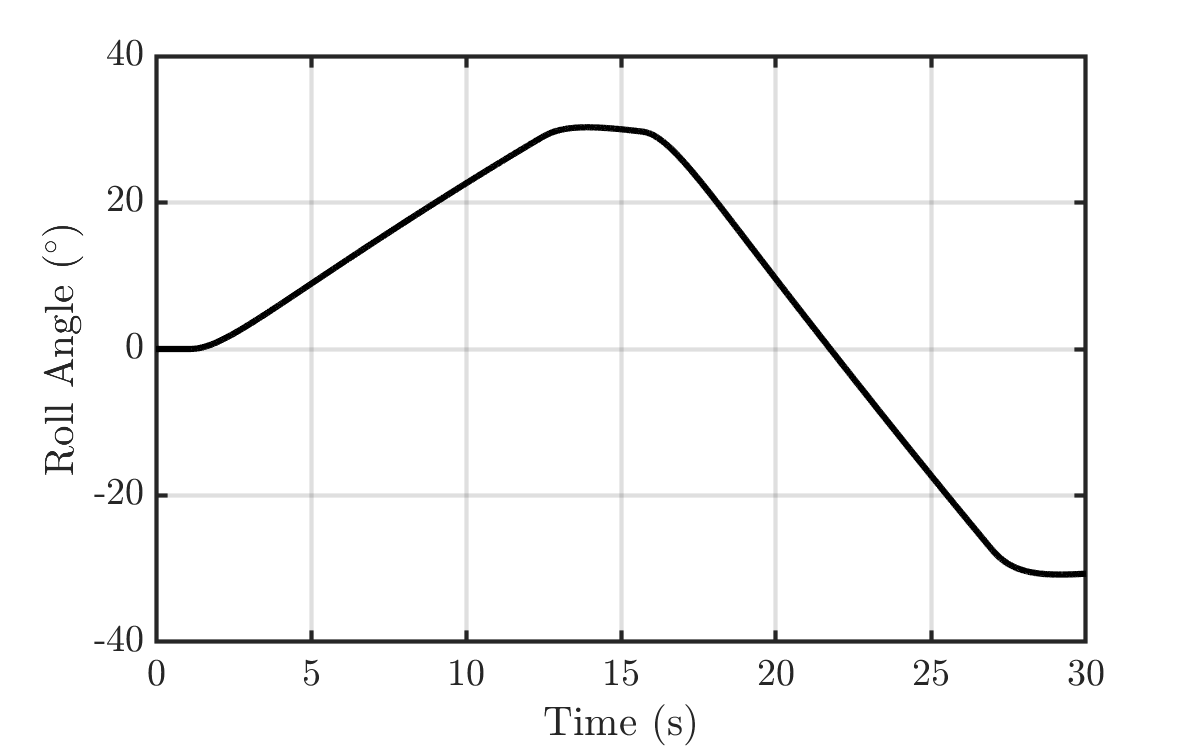
\includegraphics[trim=0 0 0 0, clip, width=.55\textwidth]{code/image_gen/cba/images/cfr147d_roll_angle.png}
        \label{subfig:roll_angle}
    }
    \end{subfigure}
    \hfill
    \begin{subfigure}[Roll acceleration that would be required for the aircraft to follow the roll angle trajectory]{
        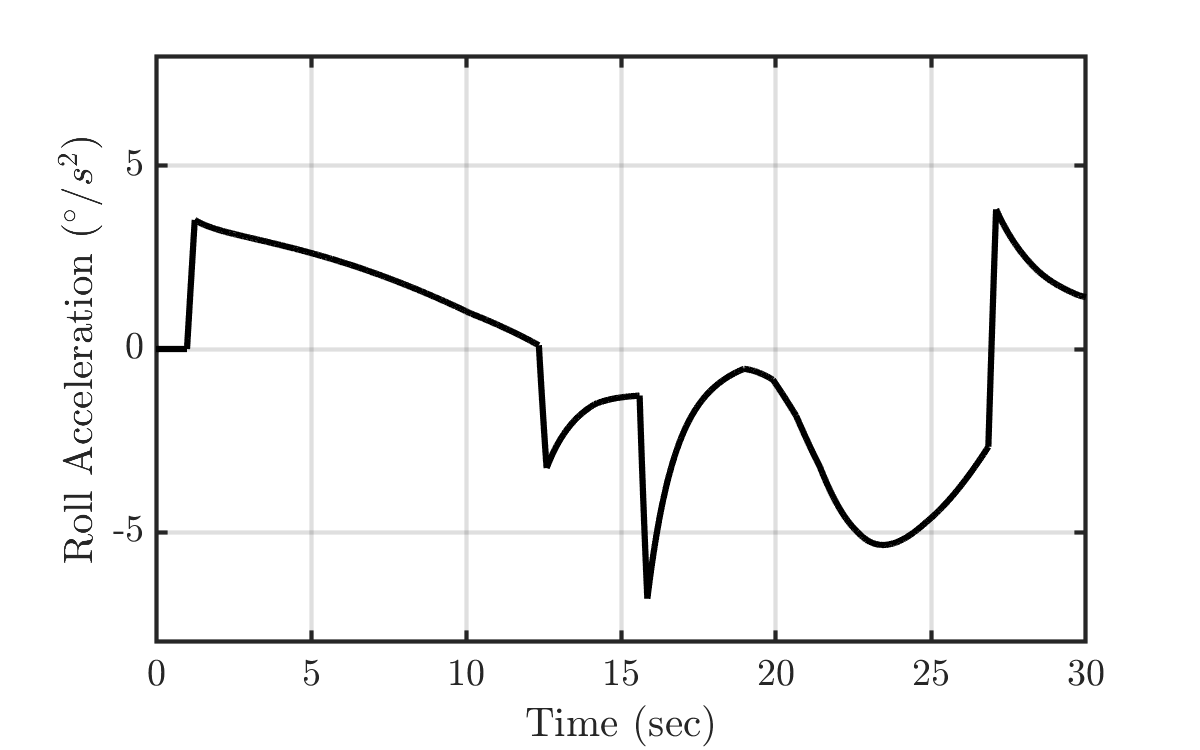
\includegraphics[trim=0 0 0 0, clip, width=.55\textwidth]{code/image_gen/cba/images/cfr147d_roll_acc.png} 
        \label{subfig:roll_acc}
    } 
    \end{subfigure}
    \hfill
    \begin{subfigure}[Left and right aileron deflections commanded to create the requisite roll accelerations]{
        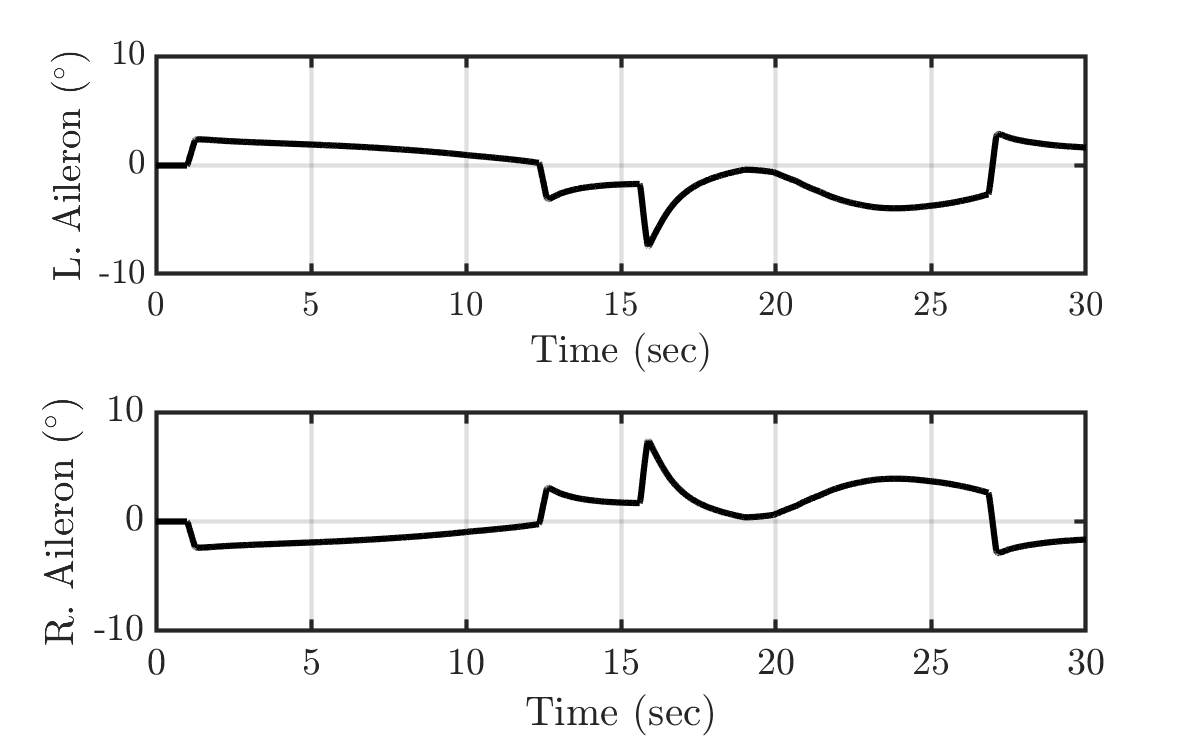
\includegraphics[trim=0 0 0 0, clip, width=.55\textwidth]{code/image_gen/cba/images/cfr147d_ail_defl.png} 
        \label{subfig:ail_defl}
    } 
    \end{subfigure}
    \caption{Flight simulation of the CFR 147(d) air-worthiness test using the GTT aircraft. \label{fig:cfr147d_inputs}}
\end{figure}

Other parameters in the trajectory definition, such as minimizing sideslip or maintaining altitude, necessitate yaw and pitch accelerations.
These are shown in Figure \ref{subfig:yaw_acc} and \ref{subfig:pitch_acc}.
In turn, these require rudder and elevator inputs that are shown in Figure \ref{subfig:rud_defl} and \ref{subfig:elev_defl}. 
Again, the linear relationship between the rotational accelerations, yawing and pitching moments, and the corresponding control surface deflections, rudder and elevator, results in the acceleration trends being closely matched by the surface deflection trends. 
As long as the surface deflections that are commanded by the flight simulator don't exceed the physical limit of the available control surface deflection, the maneuver can be completed and is considerd a success. 

\begin{figure}
    \centering
    \begin{subfigure}[Yaw acceleration required during the maneuver to minimize sideslip.] {
        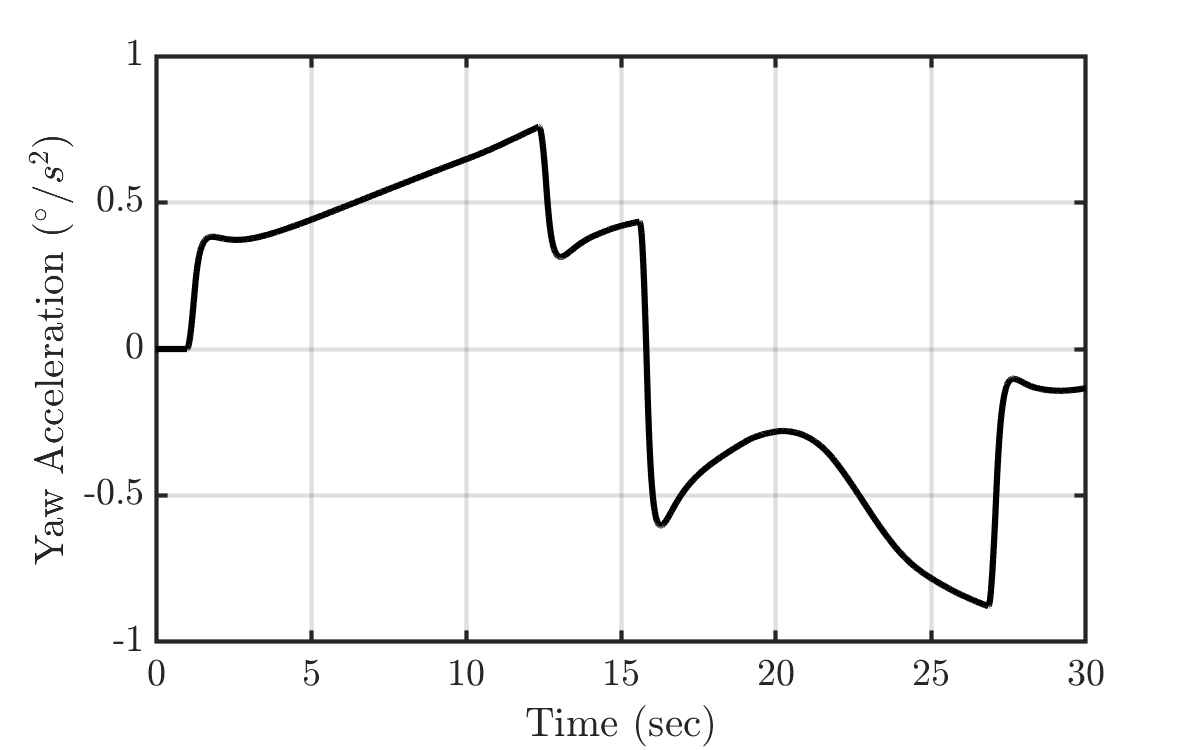
\includegraphics[trim=0 0 0 0, clip, width=.48\textwidth]{code/image_gen/cba/images/cfr147d_yaw_acc.png}
        \label{subfig:yaw_acc}
    }
    \end{subfigure}
     \hfill
    \begin{subfigure}[Pitch acceleration required during the maneuver to maintain altitude.]{
        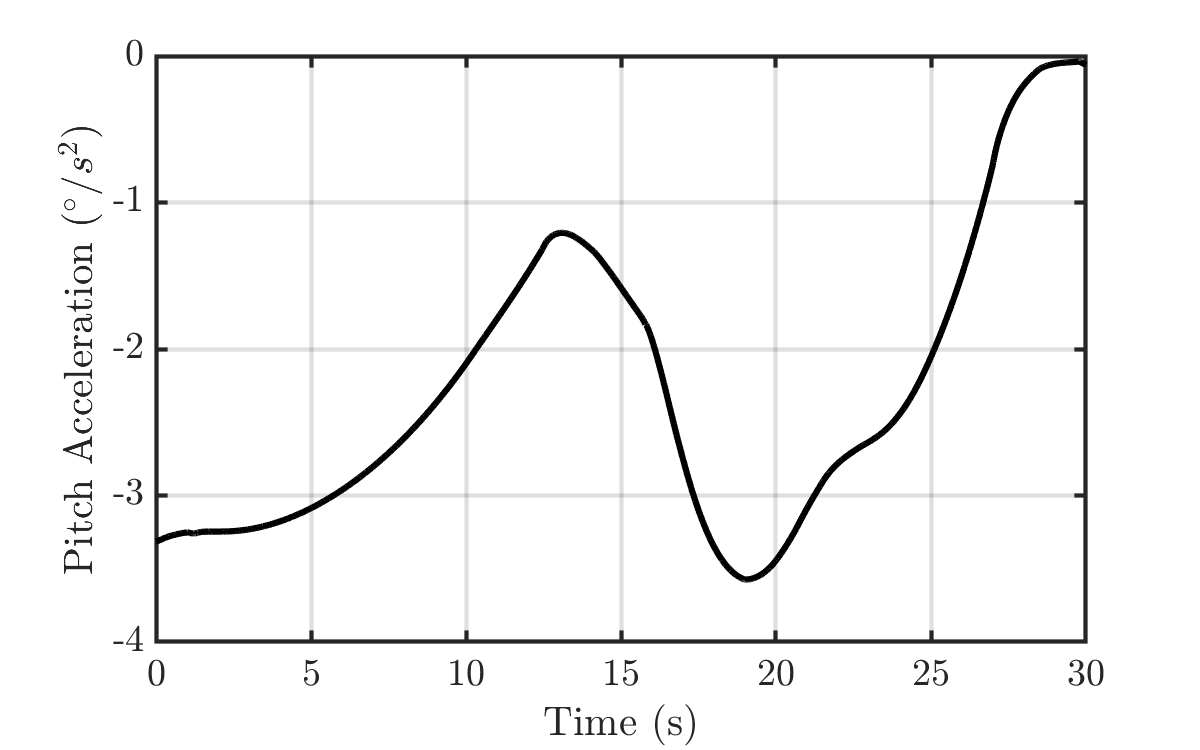
\includegraphics[trim=0 0 0 0, clip, width=.48\textwidth]{code/image_gen/cba/images/cfr147d_pitch_acc.png} 
        \label{subfig:pitch_acc}
    } 
    \end{subfigure}
    \hfill
    \begin{subfigure}[Rudder deflection required to minimize sideslip.]{
        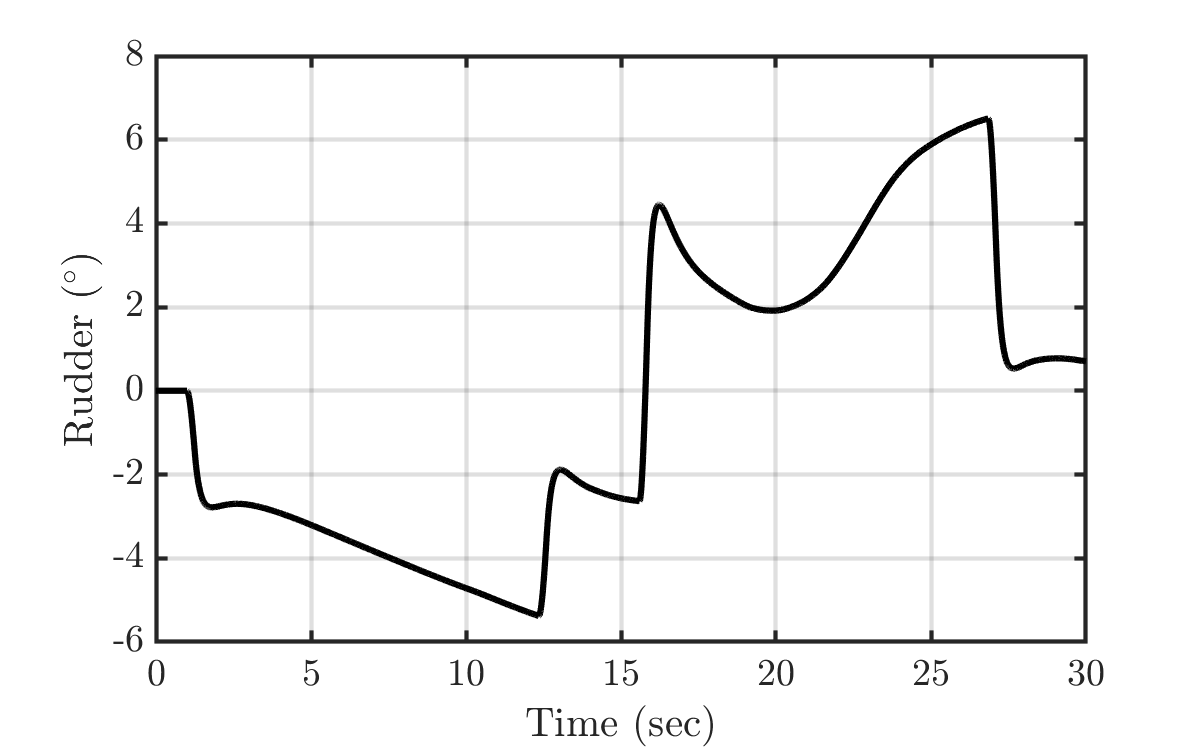
\includegraphics[trim=0 0 0 0, clip, width=.48\textwidth]{code/image_gen/cba/images/cfr147d_rud_defl.png} 
        \label{subfig:rud_defl}
    } 
    \end{subfigure}
    \hfill
    \begin{subfigure}[Elevator deflection required to maintain altitude during the banked turn.]{
        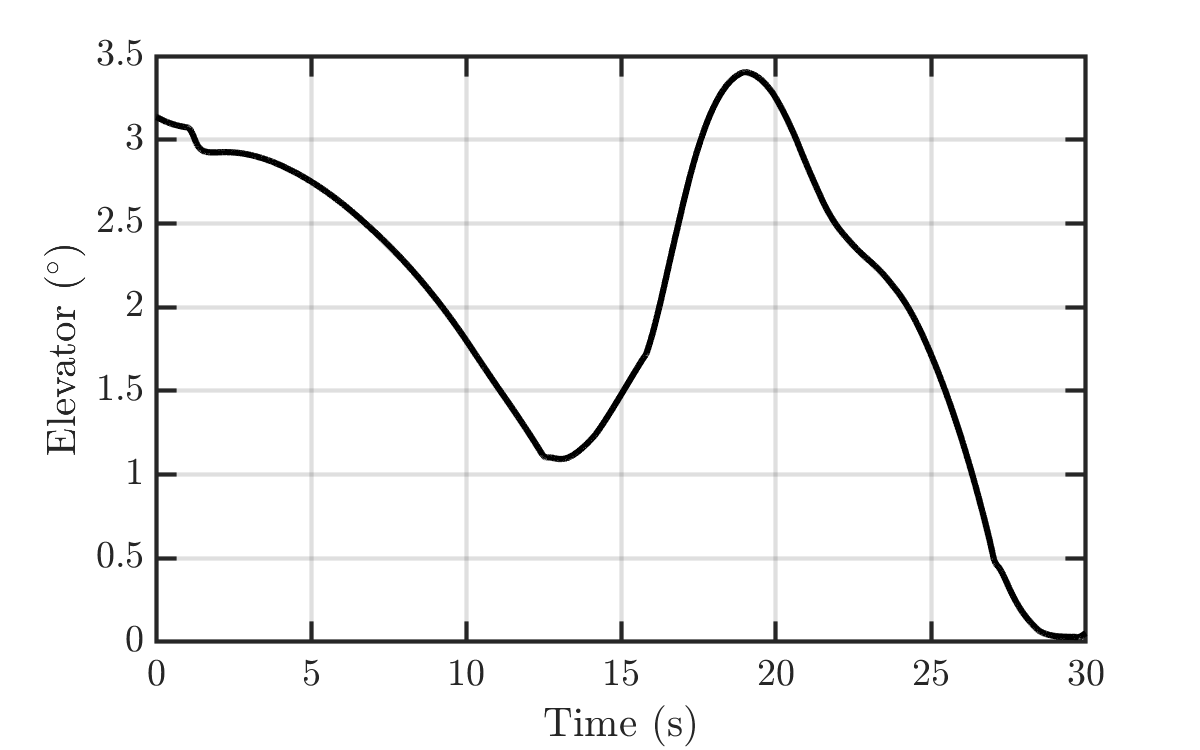
\includegraphics[trim=0 0 0 0, clip, width=.48\textwidth]{code/image_gen/cba/images/cfr147d_elev_defl.png} 
        \label{subfig:elev_defl}
    } 
    \end{subfigure}
    \caption{Rudder and elevator control inputs are required to satisfy the yaw and pitch accelerations needed to complete the maneuver.  \label{fig:cfr147d_pitch_yaw_inputs}}
\end{figure}

\subsection{Engine Failure Simulations}
As stated in Section \ref{sec:maneuver}, the certification maneuver needs to completed with one engine inoperative.
Specifically, the inoperative engine should be the one that makes the maneuver more difficult.
In the coordinate system defined by the $x$-axis pointing out of the nose and the $z$-axis pointing down towards the ground, the roll from $\psi = +30^\circ$ to $\psi = -30^\circ$ is made more difficult with the right engine inoperative. 
The asymmetric thrust causes the aircraft to yaw towards the inoperative engine, creating a rolling moment in the direction opposite to the roll maneuver.

This can be confirmed by looking at Figure \ref{fig:eo_cfr147d_inputs}. 
There are three configurations for which the time history of the rotational accelerations (left column) and the control surface deflections (right column) are plotted.
The blue line represents the nominal configuration with both engines operating. 
The red line represents the case with an inoperative right engine (Right Engine Out) and the yellow line represents the case with an inoperative left engine (Left Engine Out).
Since the engines are aligned with the $x$-axis, the asymmetric thrust does not induce any rolling moment and Figure \ref{subfig:eo_roll_acc} shows identical roll acceleration requirements for all three configurations.
However, it does induce yawing and pitching moments. 
The direction of the yawing moment depends on which engine is inoperative.
Consequently, Figure \ref{subfig:eo_yaw_acc} shows the required yaw accelerations for the engine out cases to be symmetric about the nominal condition. 
The induced pitching moment is independent of which engine is inoperative, and Figure \ref{subfig:eo_pitch_acc} confirms this with the red and yellow lines being coincident. 

Even though the roll acceleration requirements are identical, the roll-yaw coupling necessitates different aileron deflections for the different configurations, as seen in Figure \ref{subfig:eo_ail_defl}. 
Similar trends are seen for the rudder and elevator deflections in Figures \ref{subfig:eo_rud_defl} and \ref{subfig:eo_elev_defl} respectively. 
The configuration that makes the maneuver more difficult would be the one that requires higher control surface deflection angles. 
These figures show that the right engine out case (red line) requires higher aileron deflections, similar rudder deflections, and slightly higher elevator deflections. 
This confirms that having an inoperative engine on the right side of the aircraft makes the maneuver more difficult.

\begin{figure}
    \centering
    \begin{subfigure}[Roll accelerations vs. time.] {
        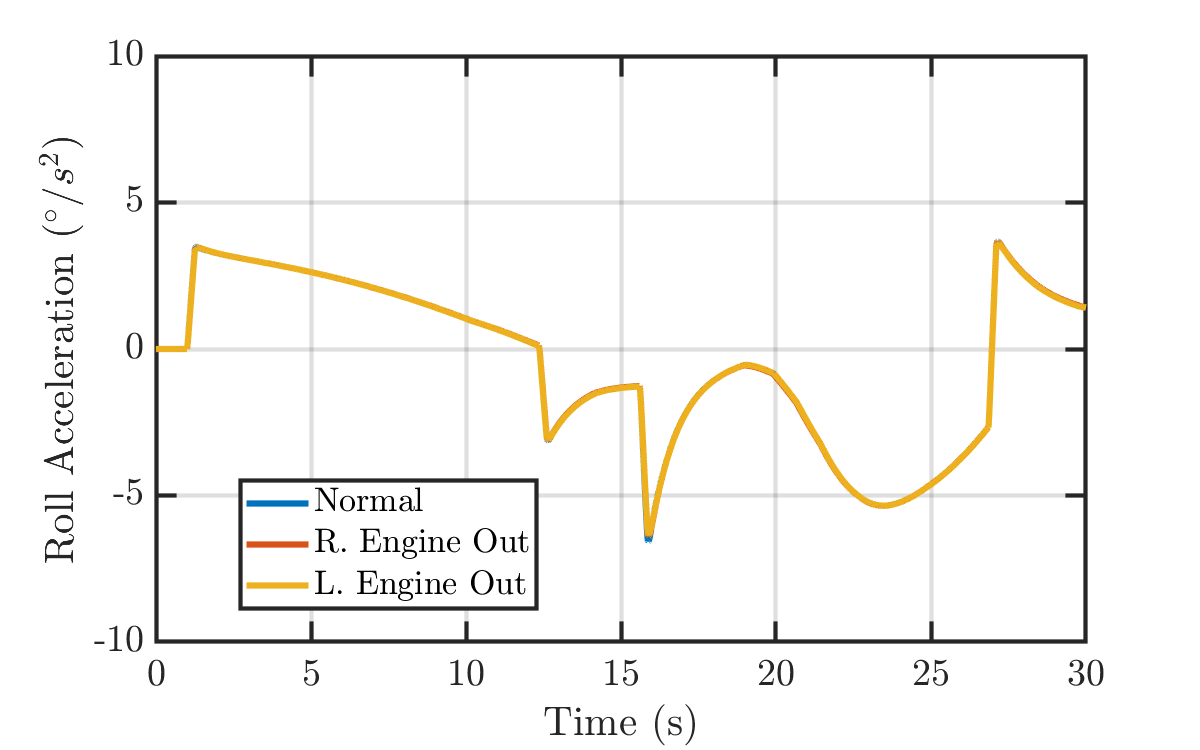
\includegraphics[trim=0 0 0 0, clip, width=.48\textwidth]{code/image_gen/cba/images/eo_cfr147d_roll_acc.png}
        \label{subfig:eo_roll_acc}
    }
    \end{subfigure}
     \hfill
     \begin{subfigure}[Aileron deflections vs. time.]{
        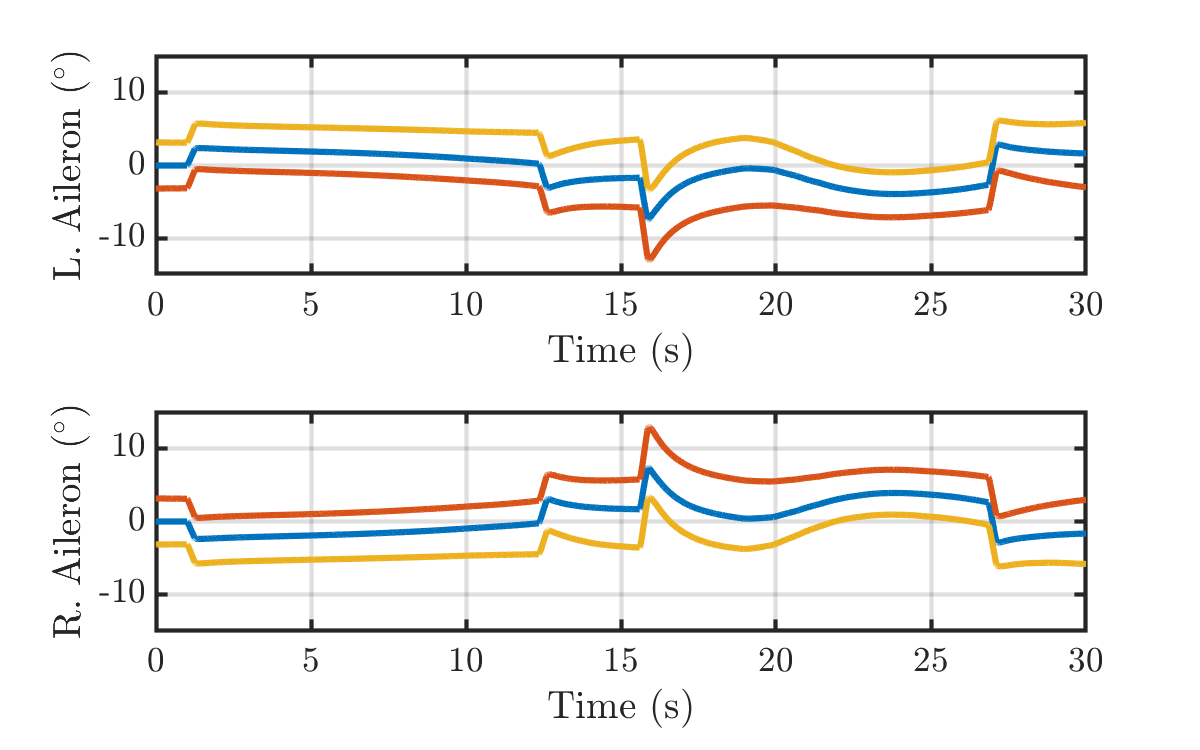
\includegraphics[trim=0 0 0 0, clip, width=.48\textwidth]{code/image_gen/cba/images/eo_cfr147d_ail_defl.png} 
        \label{subfig:eo_ail_defl}
    } 
    \end{subfigure}
    \hfill
    \begin{subfigure}[Yaw accelerations vs. time.] {
        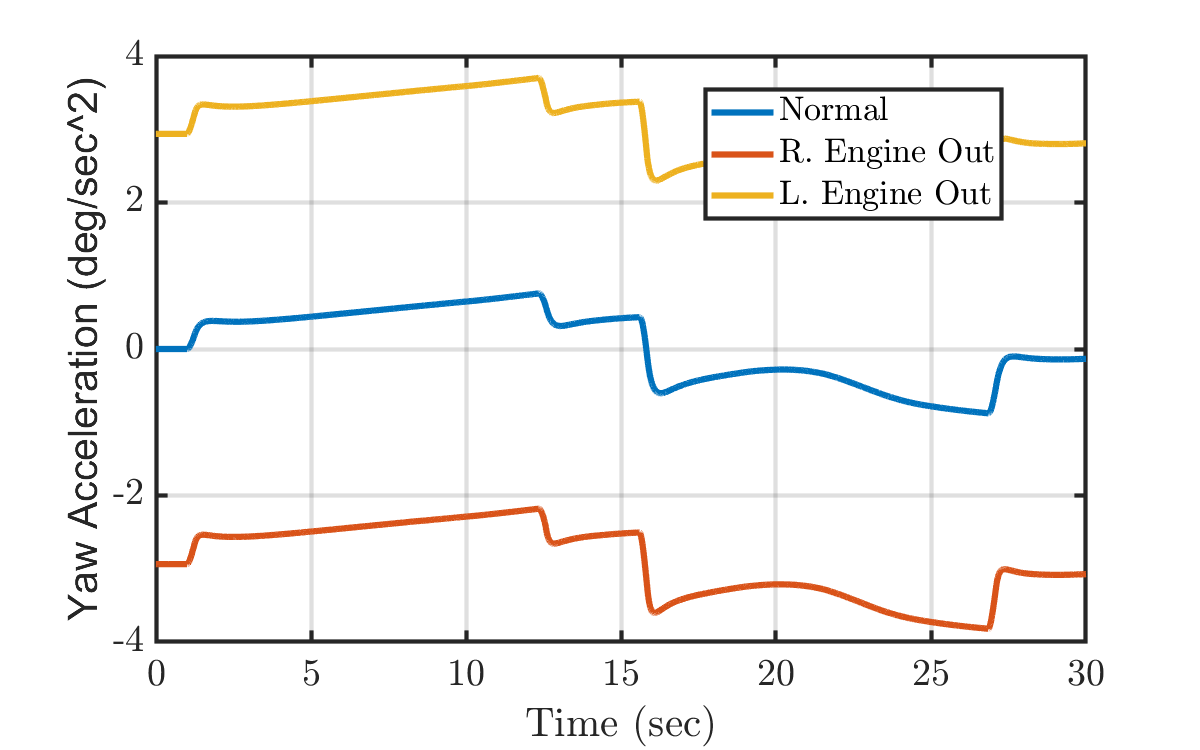
\includegraphics[trim=0 0 0 0, clip, width=.48\textwidth]{code/image_gen/cba/images/eo_cfr147d_yaw_acc.png}
        \label{subfig:eo_yaw_acc}
    }
    \end{subfigure}
    \hfill
    \begin{subfigure}[Rudder deflections vs. time.]{
        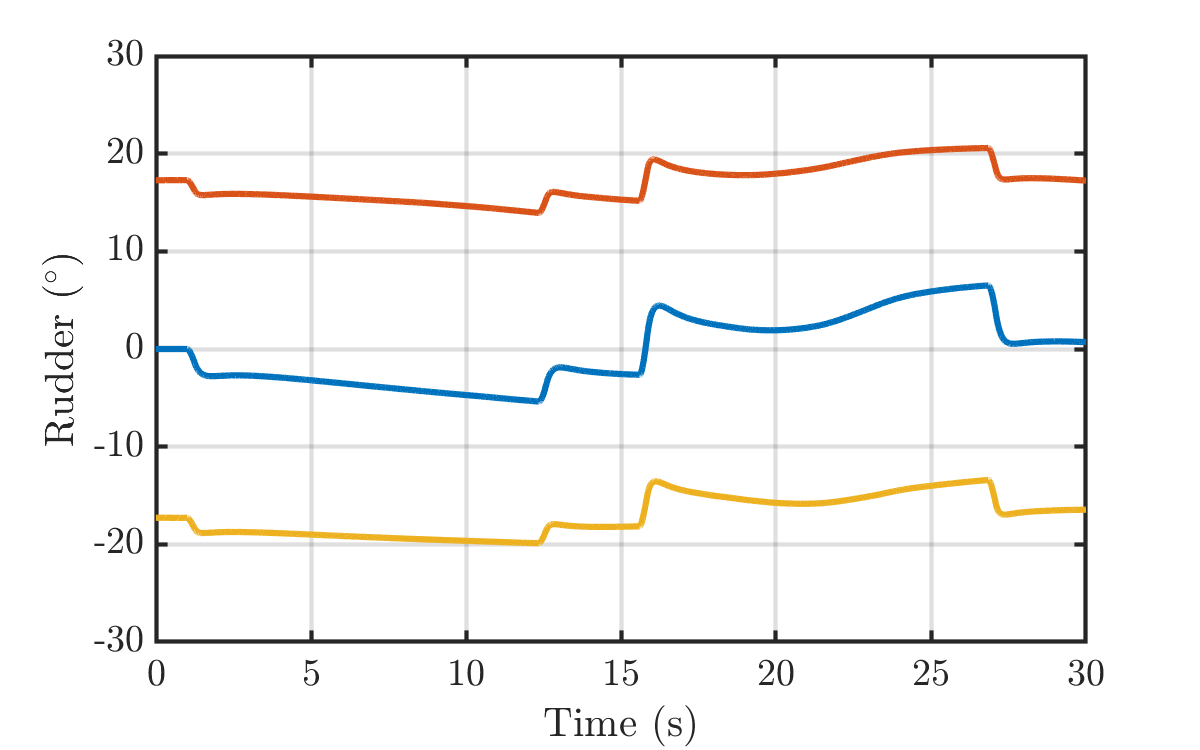
\includegraphics[trim=0 0 0 0, clip, width=.48\textwidth]{code/image_gen/cba/images/eo_cfr147d_rud_defl.png} 
        \label{subfig:eo_rud_defl}
    } 
    \end{subfigure}
     \hfill
    \begin{subfigure}[Pitch accelerations vs. time.]{
        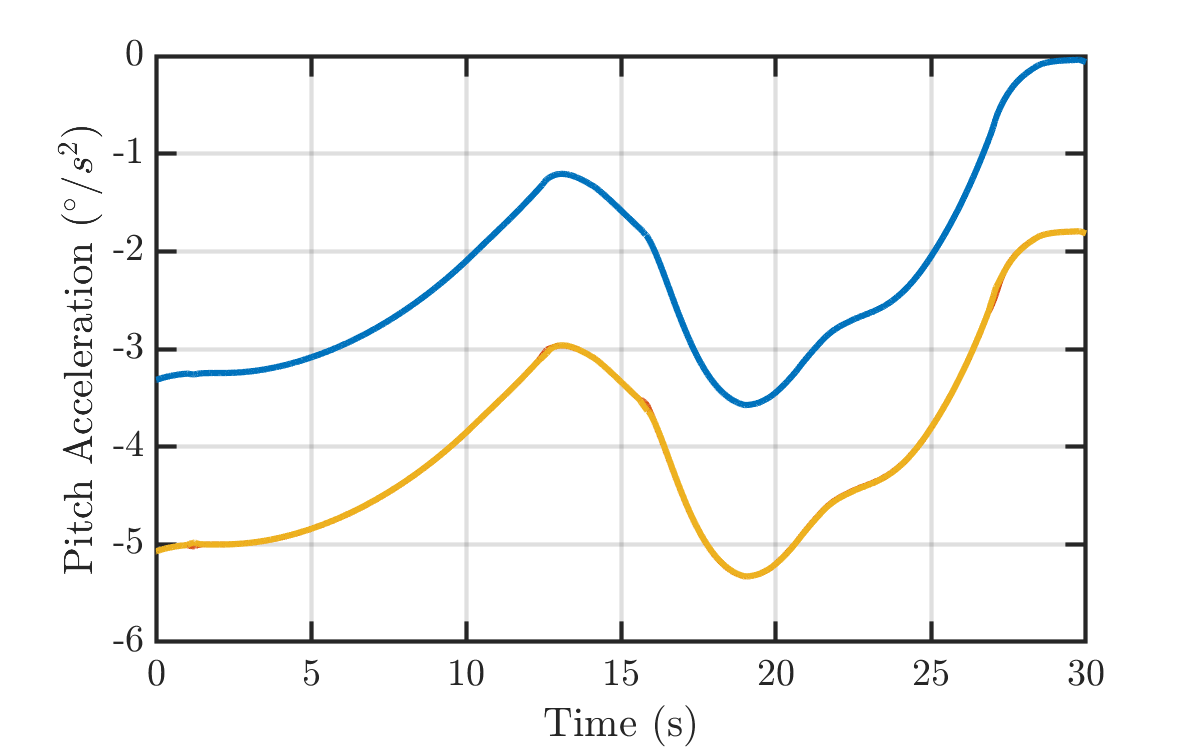
\includegraphics[trim=0 0 0 0, clip, width=.48\textwidth]{code/image_gen/cba/images/eo_cfr147d_pitch_acc.png} 
        \label{subfig:eo_pitch_acc}
    } 
    \end{subfigure}
    \hfill
    \begin{subfigure}[Elevator deflections vs. time.]{
        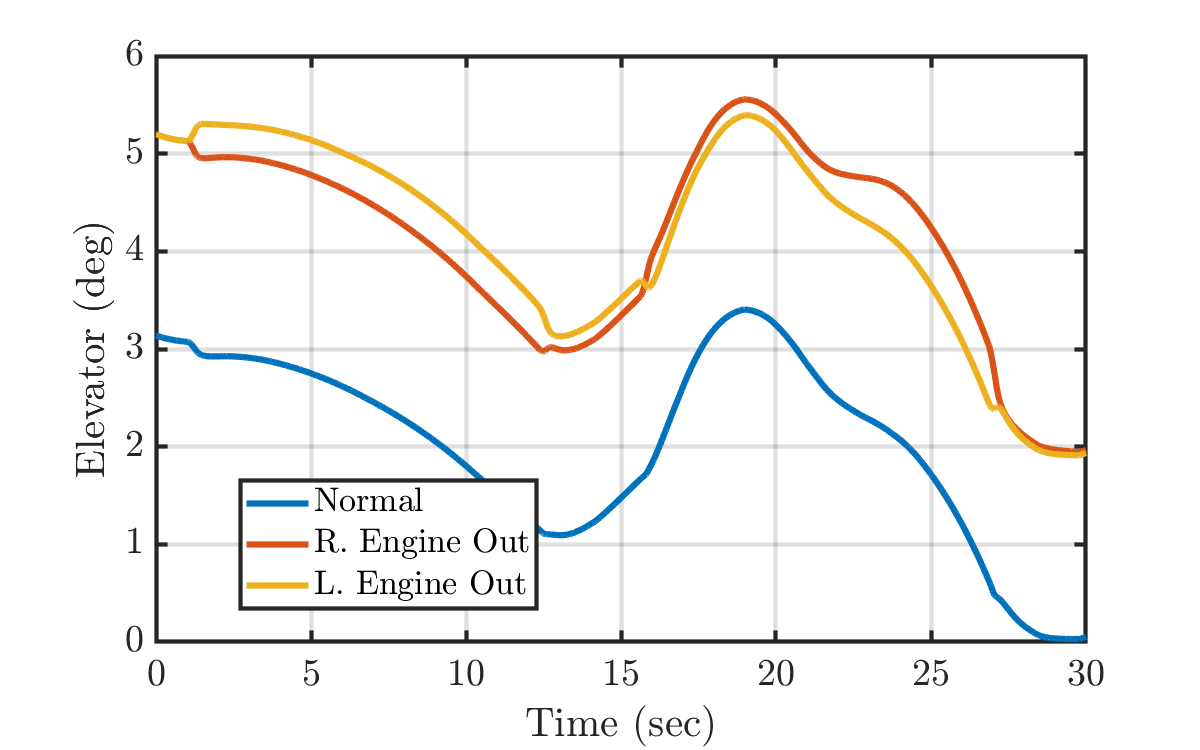
\includegraphics[trim=0 0 0 0, clip, width=.48\textwidth]{code/image_gen/cba/images/eo_cfr147d_elev_defl.png} 
        \label{subfig:eo_elev_defl}
    } 
    \end{subfigure}
    \caption{Rotational accelerations and control surface deflections required to perform the maneuver with both engines operative (blue), right engine inoperative (red), and left engine inoperative (yellow). \label{fig:eo_cfr147d_inputs}}
\end{figure}

% \subsection{Maneuver Simulation}
% Armed with the aircraft databases and the time history of the necessary control surface deflections,the flight certification maneuver can be flown using Boeing's 5DoF flight simulator. 
% At every time step during the simulation, the aircraft's state, as defined by its orientation and configuration, are tracked.
% The orientation is defined by the angle of attack and angle of sideslip of the aircraft.  
% Configuration refers to aircraft's parameters such as engine thrust, airspeed, flap position etc. 
% The aircraft's aerodynamics database defines the forces and moments that are experienced by the aircraft at that orientation and configuration. 
% The time history of the control surface deflections are translated into their resulting moments using the aircraft's controls database. 
% These forces and moments are integrated in time to calculate the aircraft's orientation and configuration at the next time step. 
% This integration in time is continued until the maneuver is complete.

% The results of one such simulation, with the right engine inoperative, can be seen in Figure \ref{fig:reo_cfr147d_sim}.
% The solid black line represents the preprocessed inputs to the simulator and the red dashed line represents a simulated maneuver.
% The simulation is able to track the trajectory and the roll accelerations exactly as shown by the coincident lines in Figures \ref{subfig:reo_roll_angle} and \ref{subfig:reo_roll_acc}. 
% Figure \ref{subfig:reo_ail_defl} shows the slight changes to the aileron deflection angles in the simulations that ensure the roll acceleration is tracked correctly.

% \begin{figure}
%     \centering
%     \begin{subfigure}[Flight simulation trajectory definition for the roll angle of the aircraft. Derived from the air-worthiness test.] {
%         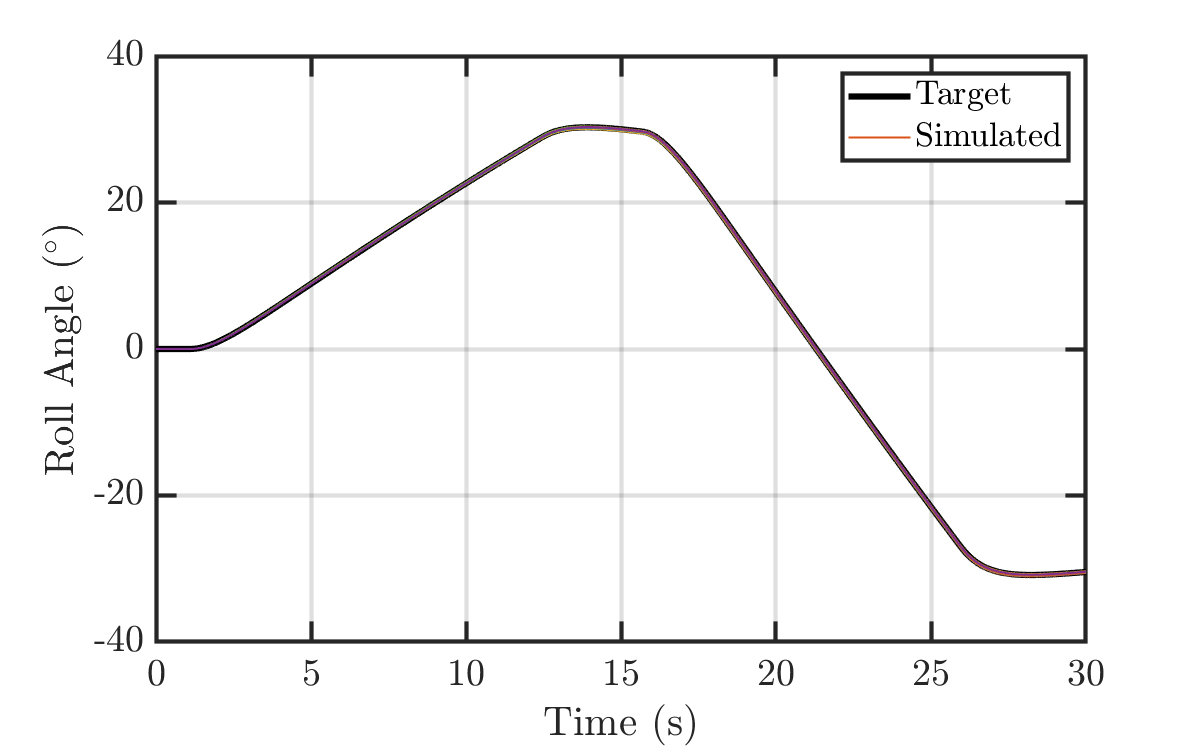
\includegraphics[trim=0 0 0 0, clip, width=.55\textwidth]{code/image_gen/cba/images/reo_cfr147d_roll_angle_mean.png}
%         \label{subfig:reo_roll_angle}
%     }
%     \end{subfigure}
%     \hfill
%     \begin{subfigure}[Roll acceleration that would be required for the aircraft to follow the roll angle trajectory]{
%         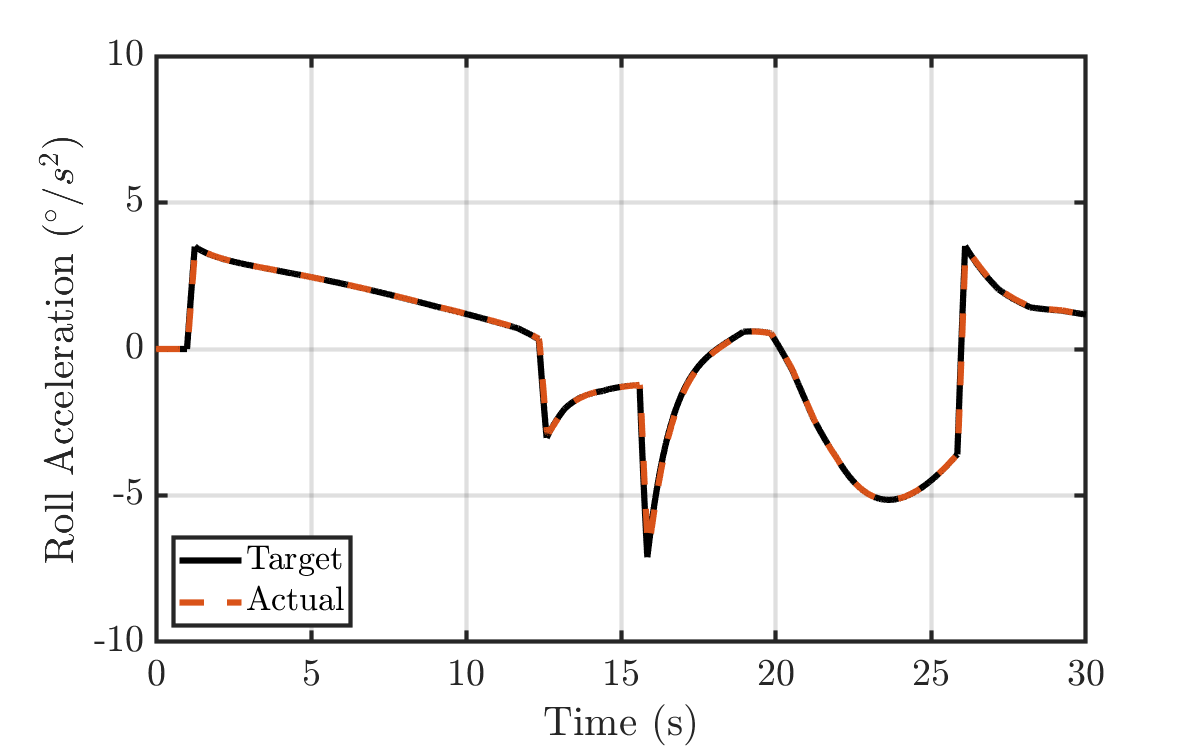
\includegraphics[trim=0 0 0 0, clip, width=.55\textwidth]{code/image_gen/cba/images/reo_cfr147d_roll_acc_mean.png} 
%         \label{subfig:reo_roll_acc}
%     } 
%     \end{subfigure}
%     \hfill
%     \begin{subfigure}[Left and right aileron deflections commanded to create the requisite roll accelerations]{
%         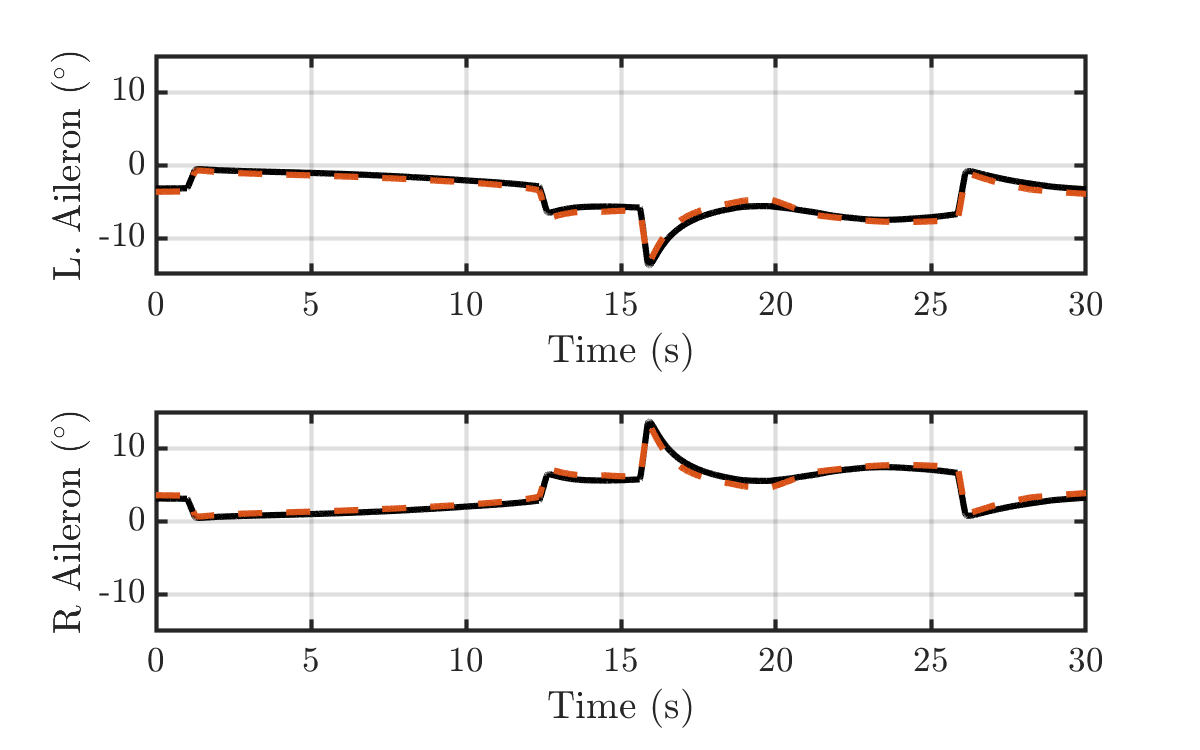
\includegraphics[trim=0 0 0 0, clip, width=.55\textwidth]{code/image_gen/cba/images/reo_cfr147d_ail_defl_mean.png} 
%         \label{subfig:reo_ail_defl}
%     } 
%     \end{subfigure}
%     \caption{Steps required to convert the air-worthiness test into a the required inputs for the flight simulation of the maneuver. \label{fig:reo_cfr147d_sim}}
% \end{figure}

\subsection{Evaluating Success or Failure} \label{subsec:success_failure}

The metric for the successful completion of the certification maneuver is defined in the FAA's guide \cite{romanowski_flight_2018} as being able to perform the $60^\circ$ change in bank angle under 11 seconds. 
Enforcing this criteria directly would require a closed-loop, trajectory-following flight simulation where the aircraft continuously calculates and adjusts the control input required to complete the maneuver as fast as possible without exceeding the physical limits on the control systems. 
In the flight simulation procedure that is used, the time taken to complete the maneuver is predefined.
There is very little variation in actual time taken for the aircraft to complete the maneuver because the control inputs are specifically calculated to complete the maneuver in the predefined time.

To work around this, the metric for success is re-framed. 
Since the time to complete the maneuver is predefined, the metric of success becomes the level of saturation of the control surfaces required to complete the maneuver. 
Specifically, three success metrics are defined, one for each rotational acceleration: pitch, roll, yaw. 
These are calculated for a simulated maneuver as
\begin{align}
    \rho_{pitch} = 1- \max\left \{ \frac{\left \vert \delta_e^{req}(t) \right \vert }{\delta_e^{lim}} \right \}
    \\
    \rho_{roll} = 1- \max\left \{ \frac{\left \vert \delta_a^{req}(t) \right \vert }{\delta_a^{lim}} \right \}
    \\
    \rho_{yaw} = 1- \max\left \{ \frac{\left \vert \delta_r^{req}(t) \right \vert }{\delta_r^{lim}} \right \}
\end{align}
where $\delta_e$, $\delta_a$, and $\delta_r$ correspond to elevator, aileron, and rudder deflection angles, respectively.
The superscript $req$ indicates the value that is calculated by the simulator, and the superscript $lim$ indicates the maximum allowable control surface deflection angle. 
The maximum saturation over the entire duration of the flight simulation is taken and subtracted from $1$.
If at any point during the flight simulation a control surface is completely saturated, say $\delta_e^{req} = \delta_e^{lim}$, the corresponding metric is $0$, in this case $\rho_{pitch} = 0$.
Consequently, a flight maneuver is considered a success if all three success metrics are $>0$.
The deflection limits for each of the control surfaces is shown in Table \ref{tab:gtt_defl_limits}.

\begin{table}
\centering
    \renewcommand{\arraystretch}{1.2}
    \captionsetup{justification=centering}
    \caption{Control surface deflection limits on the GTT aircraft.} 
    \begin{tabular}{|c|c|}
    \hline
        Control Surface & Deflection limits \\ \hline
        Ailerons & $\pm 25^\circ$ \\ \hline
        Elevator & $\pm 20^\circ$ \\ \hline
        Rudder & $\pm 30^\circ$ \\ \hline
        Spoilers & $\pm 60^\circ$ \\ \hline
        Flaps & $\pm 45^\circ$ \\ \hline
    \end{tabular}
    \label{tab:gtt_defl_limits}
\end{table}

To show a concrete example, the maneuver definition is tweaked to force the over-saturation of the ailerons.
The maneuver is made more aggressive by shortening the time taken to perform the $60^\circ$ change in bank angle from $11 sec$ to $2.5 sec$.
The maneuver trajectory, required roll accelerations, and simulated control surface deflections for the aggressive maneuver are shown in Figure \ref{fig:cfr147d_agg} as the solid blue lines. 
This is contrasted with the original maneuver in the solid black lines. 
The aileron saturation limits of $\pm 25^circ$ are indicated in Figure \ref{subfig:agg_ail_defl} as the dashed black lines. 
Over-saturation of the aileron deflection is visible with the blue line extending past the saturation limit. 
For this case, the absolute maximum deflection angle for the right aileron is $34^\circ$ which exceeds the saturation limit by $9^\circ$
The resulting roll metric $\rho_{roll} = -0.36$

\begin{figure}
    \centering
    \begin{subfigure}[Trajectory definitions for aggressive maneuver compared to that for the original certification maneuver.] {
        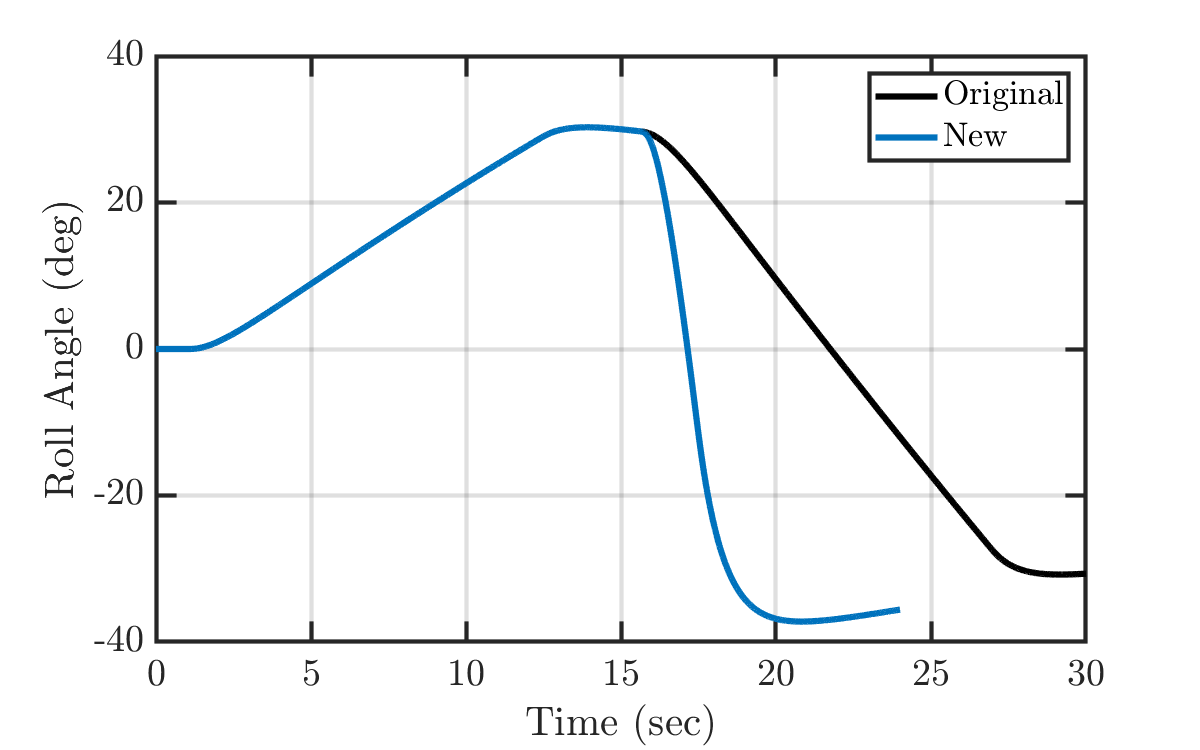
\includegraphics[trim=0 0 0 0, clip, width=.55\textwidth]{code/image_gen/cba/images/cfr147d_agg_roll_angle.png}
        \label{subfig:agg_roll_angle}
    }
    \end{subfigure}
    \hfill
    \begin{subfigure}[Roll accelerations that would be required for the two maneuvers]{
        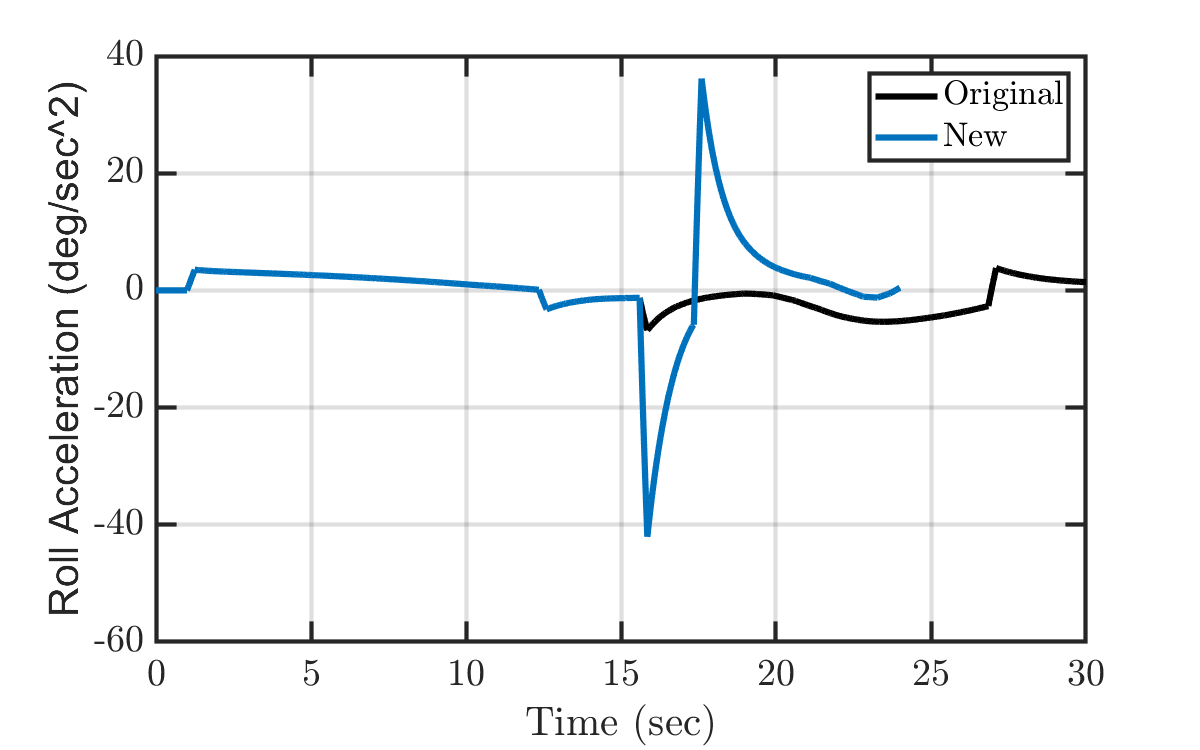
\includegraphics[trim=0 0 0 0, clip, width=.55\textwidth]{code/image_gen/cba/images/cfr147d_agg_roll_acc.png} 
        \label{subfig:agg_roll_acc}
    } 
    \end{subfigure}
    \hfill
    \begin{subfigure}[Left and right aileron deflections needed to perform the two maneuvers.]{
        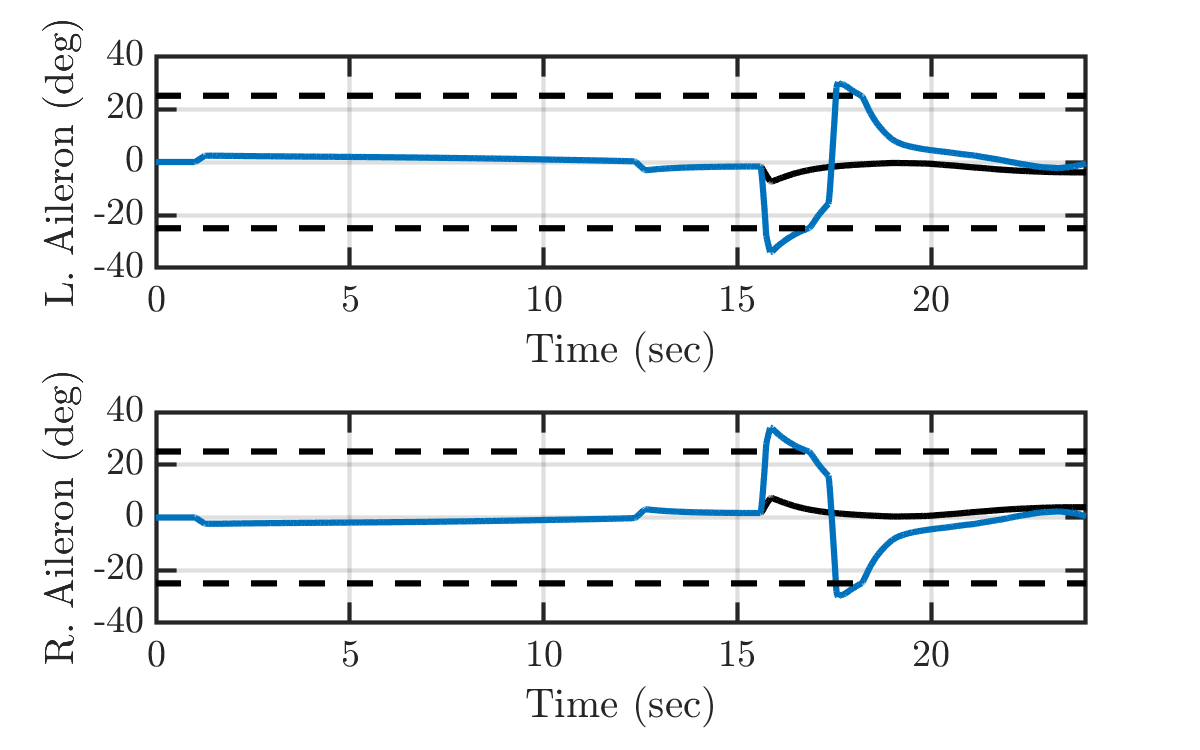
\includegraphics[trim=0 0 0 0, clip, width=.55\textwidth]{code/image_gen/cba/images/cfr147d_agg_ail_defl.png} 
        \label{subfig:agg_ail_defl}
    } 
    \end{subfigure}
    \caption{Comparing the results of performing an aggressive roll maneuver that over-saturates the aileron control authority (solid blue line) vs. those of performing the original certification maneuver. Note the over-saturation of the ailerons for the aggressive maneuver. \label{fig:cfr147d_agg}}
\end{figure}

It is important to note that aircraft analysis data is only available within the saturation limits of the control surfaces. 
When the simulator commands a control surface deflection that is greater than the limit, it is estimating the effect of that deflection by extrapolating from the provided data. 
While this extrapolation might be prone to error, it does provide an estimate for how much additional control authority would be required to complete the maneuver as planned. 

This highlights an advantage of using this simulation method and the control-surface-based metrics in the design process. 
When running a potential aircraft design through this virtual flight testing framework, the metrics provide a direct estimation of the amount of additional control authority that would be required to complete the maneuver successfully. 
If a simulation yields $\rho_{roll} = -0.25$, that means that the aircraft would require $25\%$ more aileron control authority. 
This could be achieved by increasing the control surface deflection limits by $25\%$, or by increasing the size of the ailerons. 
Additionally, by breaking up the calculations of the accelerations and the control surface deflections, different control laws can be tested without having to repeat the first step of the simulation. 
Perhaps instead of increasing the size of the aileron, greater spoiler deflections can be mixed into the control law, which would serve the same purpose of increasing the control authority in the roll direction. 

\subsection{Monte Carlo Analysis}

The GP models provide a probabilistic representation of the aerodynamics and controls databases. 
Random sampling from these models creates instances of the databases that have slight variations that are dependent on the uncertainties present in the GP model.
The sampling methodology is explained in Section \ref{sec:gpr} using Equation \ref{equ:gp_sampling}.
Each sample can be run through the flight simulator independently.
Using the original flight certification maneuver with the right engine inoperative, the results of running 10 aircraft samples through the flight simulator are shown in Figure \ref{fig:cfr147d_mc}.
As mentioned before, a single-fidelity GP trained on all the wind tunnel data is used for these results. 
The roll acceleration and the aileron deflections for the database that represents the GP model's mean prediction, is shown as a solid black line. 
The results of the samples are the individual colored lines. 
The variations in the aerodynamic databases results in varied acceleration requirements, as seen in Figure \ref{subfig:roll_acc_mc}.
These differences are compounded upon in the next step, where variations in the controls databases result in varied control surface deflection requirements (Figure \ref{subfig:ail_defl_mc}.
Each simulation results in new set of success metrics. 

\begin{figure}
    \centering
    \begin{subfigure}[Roll acceleration vs. time]{
        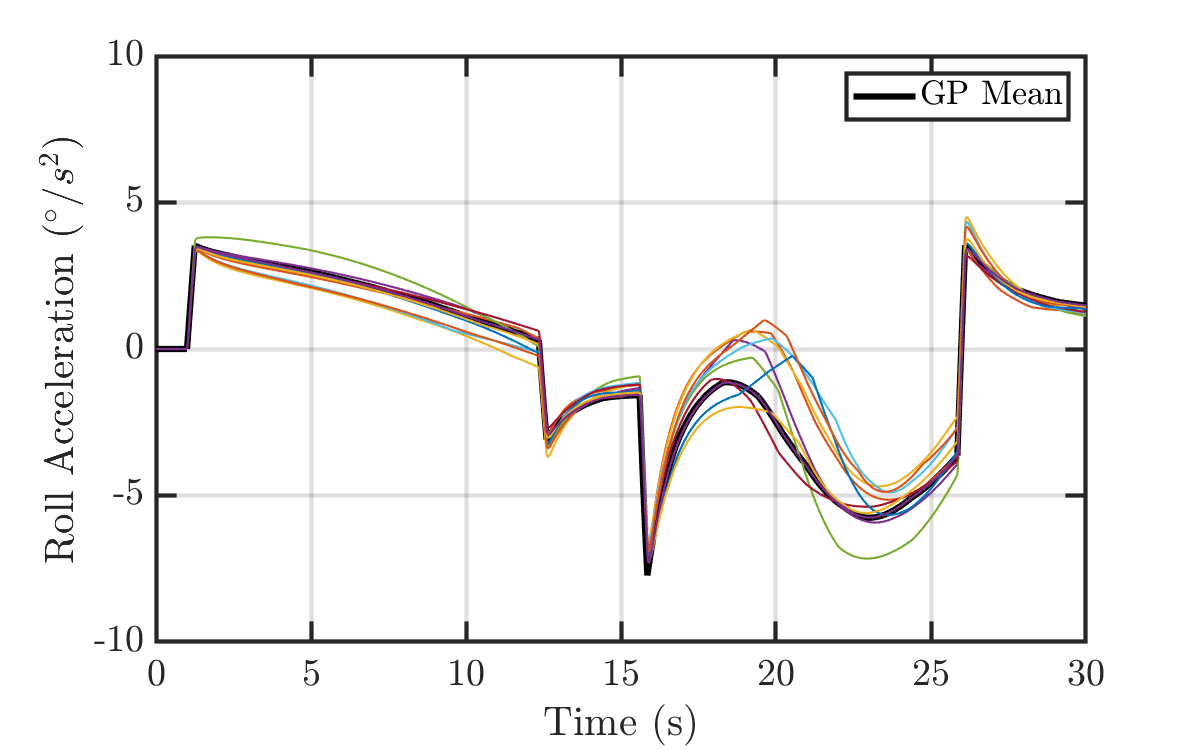
\includegraphics[trim=0 0 0 0, clip, width=.48\textwidth]{code/image_gen/cba/images/reo_cfr147d_roll_acc_mc.png} 
        \label{subfig:roll_acc_mc}
    } 
    \end{subfigure}
    \hfill
    \begin{subfigure}[Left and right aileron deflections vs. time]{
        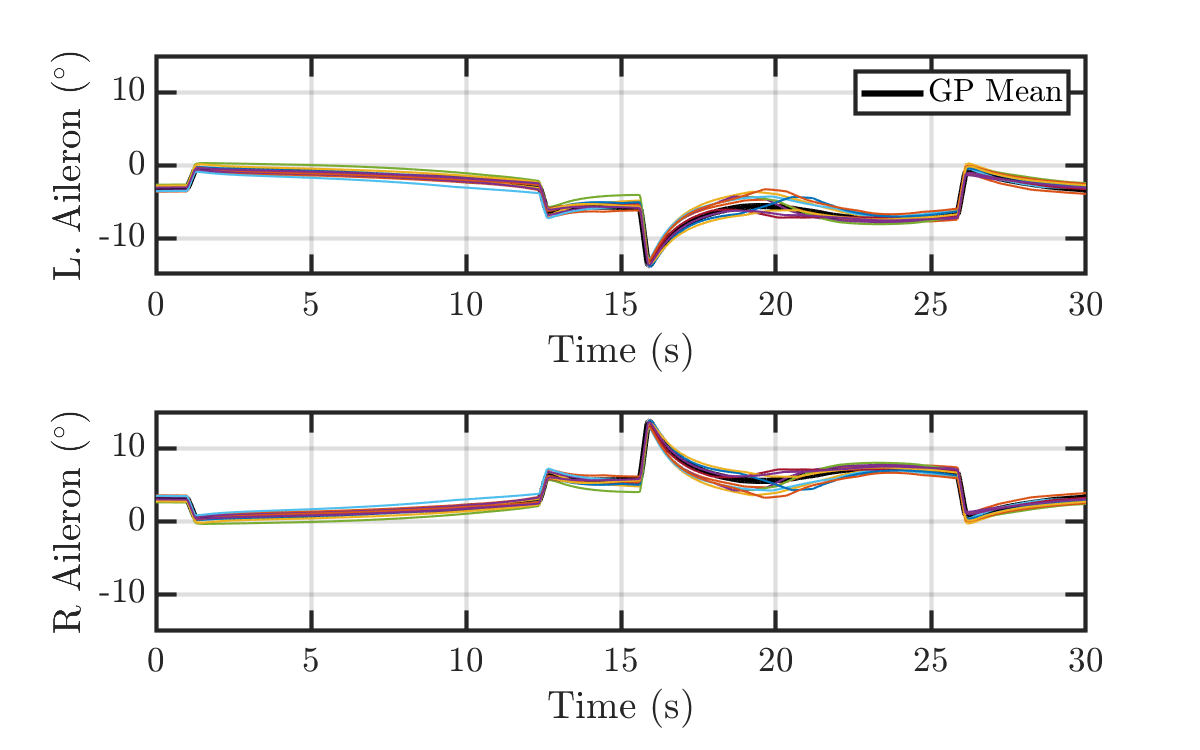
\includegraphics[trim=0 0 0 0, clip, width=.48\textwidth]{code/image_gen/cba/images/reo_cfr147d_ail_defl_mc.png} 
        \label{subfig:ail_defl_mc}
    } 
    \end{subfigure}
    \caption{Results of running 10 samples of the aerodynamics and controls databases for the GTT aircraft. Each sample exhibits small variations on the mean results.  \label{fig:cfr147d_mc}}
\end{figure}

To rigorously understand the effect of the uncertainties in the databases on the certification of the aircraft, the Monte Carlo method is used. 
This is a brute-force method of characterizing the effect of input uncertainties on an output quantity of interest (QoI), where independently, randomly sampled inputs are run through the function in question, so that the distribution of the output QoI can be studied. 
In the context of this work, the input uncertainty is the uncertainty in the analysis data that is used to create the GP models. 
The function in question is the simulation of the flight certification maneuver.
The output QoI is the success/failure of the aircraft in performing a flight certification maneuver, which is quantified by the metrics introduced in Section \ref{subsec:success_failure}.
Running flight simulations on hundreds of randomly sampled databases results in hundreds of success metrics which can be treated as a random variable as well.
Statistical methods can then be used to characterize the distribution of the success metrics. 

For the statistical analysis of the success metrics, cumulative distribution functions (CDF) are calculated.
The CDF for a random variable $X$ evaluated at $x$ represents the probability that $X$ will take a value less than or equal to $x$.
As a concrete example, $1000$ samples of the GTT aerodynamics and controls databases are used to perform the flight certification maneuver with engine failures. 
The CDF of each metrics for each engine-out situation is shown in Figure \ref{fig:mc_metric_cdfs}.
The solid lines represent the CDF for the metric, while the dashed vertical lines indicate the metric value for the simulation run with the mean GP databases.
There are a few trends that are worth pointing out that will also help in reading these, and subsequent CDF plots:

\begin{enumerate}
    \item For the pitch metric, Figure \ref{subfig:mc_pitch_cdf},
    \begin{enumerate}
        \item Clustering of the three CDF indicates that the engine operation does not affect the control authority of the aircraft in pitch.
        \item The high pitch metric values indicates that very little of the elevator's full range-of-motion is needed to complete the maneuver.
    \end{enumerate}
    \item For the roll metric, Figure \ref{subfig:mc_roll_cdf},
    \begin{enumerate}
        \item The lower roll metric values of the right engine out case (REO) indicates that larger aileron deflections, when compared to the other cases, are required to perform the maneuver.
        \item The REO case also has a larger spread of values, indicating more variance in the simulation results
        \item Higher roll metric values for the left engine out case (LEO) means that it is less demanding on the ailerons than the nominal case with both engines operative. 
    \end{enumerate}
    \item For the yaw metric, Figure \ref{subfig:mc_yaw_cdf},
    \begin{enumerate}
        \item The nearly vertical CDF plots indicate very low variance in the simulation results.
        \item Once again, the REO case is the most restrictive, requiring the largest rudder deflections to complete the maneuver. 
    \end{enumerate}
\end{enumerate}

\begin{figure}
    \centering
    \begin{subfigure}[CDF for the pitch metric]{
        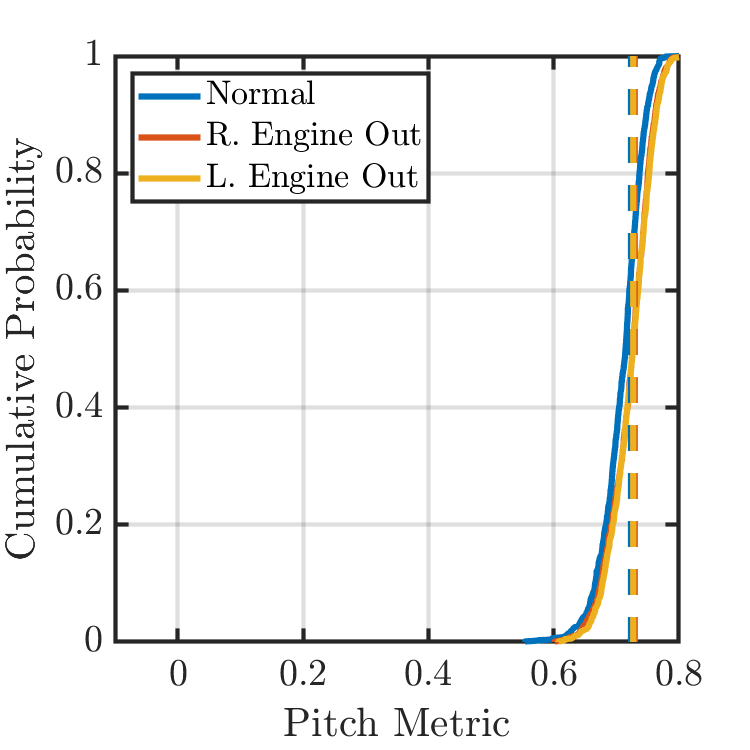
\includegraphics[trim=0 0 0 0, clip, width=.31\textwidth]{code/image_gen/cba/Stanford_CFR25_147d_2_R2/images/orig_pitch_metric_1000.png} 
        \label{subfig:mc_pitch_cdf}
    } 
    \end{subfigure}
    \hfill
    \begin{subfigure}[CDF for the roll metric]{
        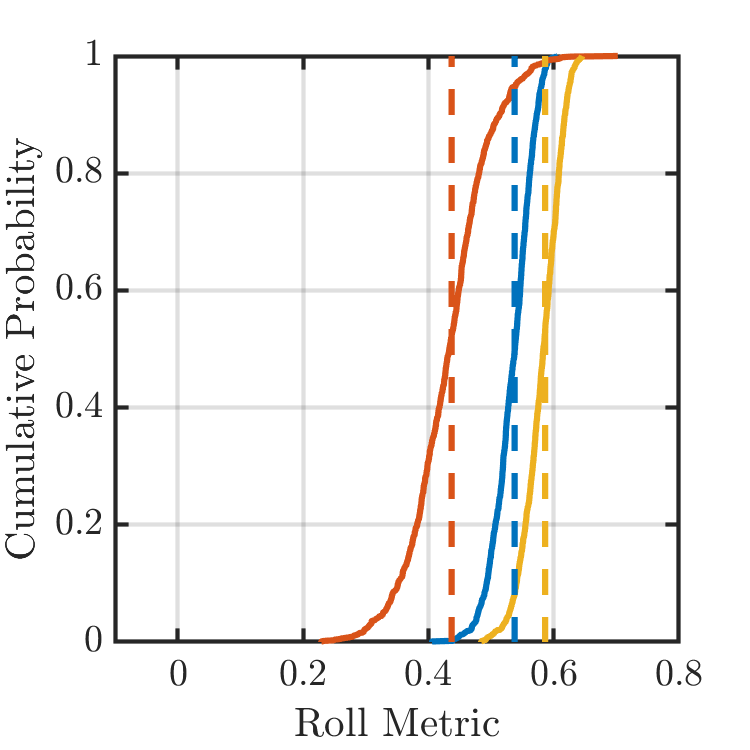
\includegraphics[trim=0 0 0 0, clip, width=.31\textwidth]{code/image_gen/cba/Stanford_CFR25_147d_2_R2/images/orig_roll_metric_1000.png} 
        \label{subfig:mc_roll_cdf}
    } 
    \end{subfigure}
    \hfill
    \begin{subfigure}[CDF for the yaw metric]{
        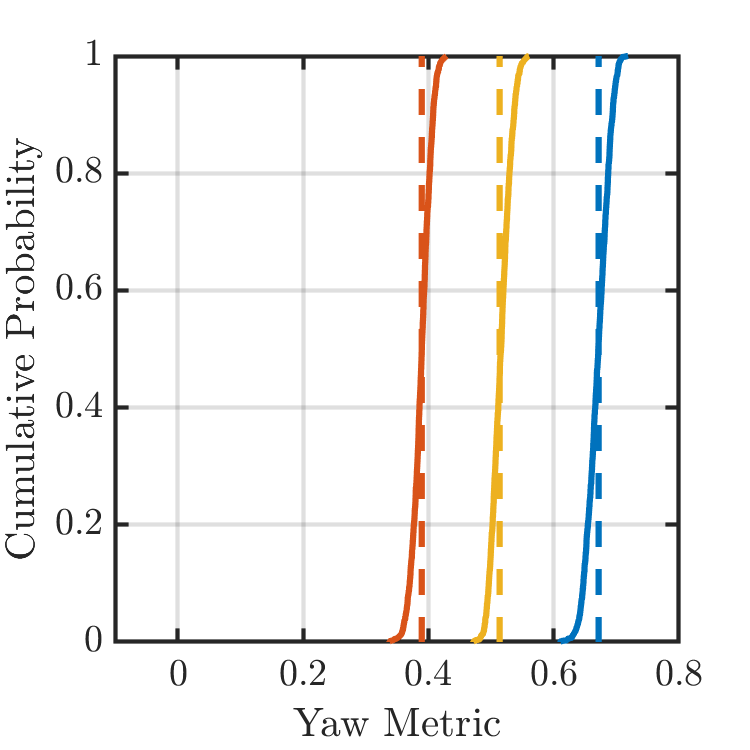
\includegraphics[trim=0 0 0 0, clip, width=.31\textwidth]{code/image_gen/cba/Stanford_CFR25_147d_2_R2/images/orig_yaw_metric_1000.png} 
        \label{subfig:mc_yaw_cdf}
    } 
    \end{subfigure}
    \caption{CDF plots for the success metrics when 1000 samples of the aerodynamics and controls databases for the GTT aircraft are used to simulate the flight certification maneuver. \label{fig:mc_metric_cdfs}}
\end{figure}

None of the metrics for any of the simulations go below $0$. 
The current representation of the aircraft, even when accounting for uncertainties in the analyses, would pass the certification maneuver $100\%$ of the time.
This is to be expected since the GTT aircraft is modeled on the CRJ 700, a currently certified aircraft.
These plots reiterate the conclusion that the REO case is the most restrictive for the certification. 
All remaining results will only use the REO case for the simulations. 

With Monte Carlo simulations, it is imperative that enough samples are used to ensure that the posterior distributions are converged.
The convergence of the distribution can be tracked using the variance of the metrics.
Figure \ref{fig:mc_var_conv} plots the variance of the roll metric distributions with increasing numbers of samples.
While the REO case takes longer to converge, the variance is unchanging by the time $1000$ samples are used. 
For this reason, all remaining results will use $1000$ Monte Carlo samples to represent the CDF for the simulation results. 

\begin{figure}
    \center
    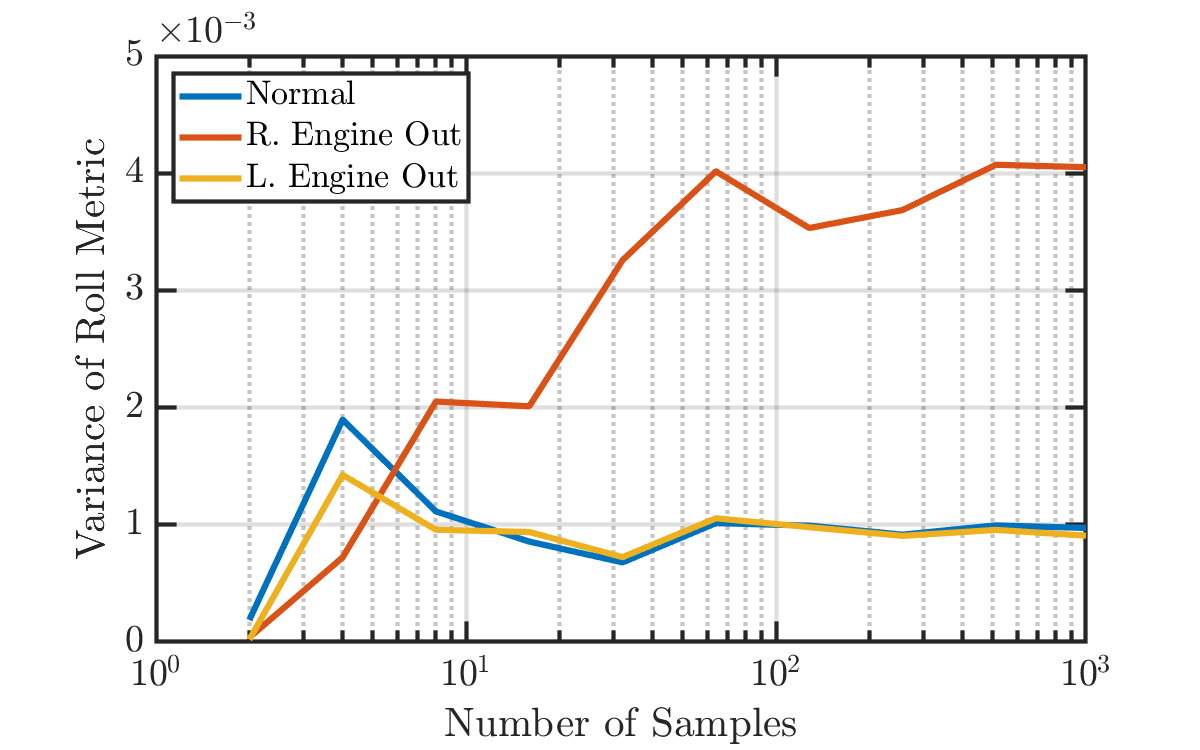
\includegraphics[width=0.65\textwidth]{code/image_gen/cba/Stanford_CFR25_147d_2_R2/images/mc_var_convergence.png}
    \caption{Convergence of the variance with increasing Monte Carlo samples \label{fig:mc_var_conv}}
\end{figure}

\subsection{Modifications to the Simulation} \label{subsec:sim_mods}

From the metric plots in the previous section, Figure \ref{fig:mc_metric_cdfs}, it is evident that the GTT aircraft can pass the flight certification maneuver $100\%$ of the time.
This is true even when the uncertainties in the analyses are taken into account in the GP model. 
It makes the discussion of success/failure of a certification maneuver difficult if the aircraft succeeds every time.
Having presented the results of the standard flight simulation in the previous section, some modifications to the simulation are made to force some failures in the maneuvers.
To make the maneuver more challenging, the limits on the control surfaces are changed.
The changes are presented in Table \ref{tab:gtt_defl_limits_new}.

The aileron and rudder limits are made more restrictive. 
These have the direct impact of increasing the control surface saturation, thereby moving the roll and yaw metrics closer towards $0$.
Spoilers aid in the roll authority and are not used moving forward.
Since flaps affect the baseline aerodynamics and lower fidelity methods are not able to model them well, they are also ignored moving forward. 
This impacts the pitch metric indirectly. 
Without flap deployment, the $C_L$ of the aircraft at all angles of attack is reduced consequently forcing the aircraft to trim at a higher angle of attack to maintain steady level flight. 
This increases dependence on the elevator during the maneuver and shifts the pitch metric closer towards $0$.

\begin{table}
\centering
    \renewcommand{\arraystretch}{1.2}
    \captionsetup{justification=centering}
    \caption{New control surface deflection limits on the GTT aircraft.} 
    \begin{tabular}{|c|c|c|}
    \hline
        Control surface & Old deflection limits & New deflection limits \\ \hline
        Ailerons & $\pm 25^\circ$ & $\pm 15^\circ$ \\ \hline
        Elevator & $\pm 20^\circ$ & $\pm 20^\circ$ \\ \hline
        Rudder & $\pm 30^\circ$ & $\pm 20^\circ$   \\ \hline
        Spoilers & $\pm 60^\circ$ & Not Used       \\ \hline
        Flaps & $\pm 45^\circ$ & Not used          \\ \hline
    \end{tabular}
    \label{tab:gtt_defl_limits_new}
\end{table}